\documentclass [12pt] {oblivoir}

\usepackage{fapapersize}
\usefapapersize{210mm,297mm,20mm,*,20mm,22mm}

\setlength\parindent{0pt}

\usepackage{graphicx}
\usepackage{mathtools}
\usepackage{amsmath}
\usepackage{upgreek}

\begin{document}
아래 그림에서 보인 것처럼 장애물이 놓인 길을 따라 공을 오른쪽으로 굴릴 때, 공의 중심이 어떤 궤적을 따라 이동하는지 알고자 한다.

길에 놓인 장애물들은 직사각형으로 표시되고, 모든 장애물은 $x$ 축 상에 놓여있다.

공이 장애물을 만나 더 이상 움직일 수 없다면 그림에서 보듯이 장애물의 벽 또는 모서리를 따라 넘어가되, 공은 어떤 경우에도 장애물에서 떨어지지 않은 채 장애물의 벽 또는 모서리를 따라 구르며, 아무리 높은 장애물도 넘어 갈 수 있다.

공의 반지름, 출발점 위치(즉, 공의 중심의 $x$ 좌표), 도착점 위치, 그리고 모든 장애물의 위치와 크기에 대한 정보가 주어질 때, 공의 중심이 이동한 총 거리를 출력하는 프로그램을 작성하고자 한다.

단, 공의 반지름을 $R$이라 하면, 모든 장애물의 너비는 $2R$ 초과이며, 또한 장애물 사이의 간격도 $2R$초과이다. 그리고 출발점과 도착점에서는 공이 항상 바닥에 닿아 있다고 가정하라.

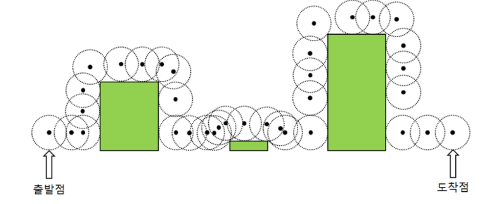
\includegraphics{n2.png}

- 제한시간: 전체 테스트 케이스는 150개 이하이며, 전체 수행 시간은 1초 이내. (Java 2초 이내)

제한 시간을 초과하면 제출한 소스코드의 프로그램이 즉시 종료되며, 그때까지 수행한 결과에서 테스트 케이스를 1개 그룹 이상 통과하였더라도 점수는 0점이 됩니다.

그러나, 제한 시간을 초과하더라도 테스트 케이스를 1개 그룹 이상 통과하였다면 '부분 점수(0 $<$ 점수 $<$ 만점)'를 받을 수 있으며,

이를 위해서는, C / C++ 에서 "printf 함수" 사용할 경우, 프로그램 시작부분에서 "setbuf(stdout, NULL);"를 한번만 사용하십시오.

C++에서는 "setbuf(stdout, NULL);"와 "printf 함수" 대신 "cout"를 사용하고, Java에서는 "System.out.printIn"을 사용하시면,

제한 시간을 초과하더라도 '부분 점수'를 받을 수 있습니다.

※ 언어별 기본 제공 소스코드 내용 참고

만약, 제한 시간을 초과하지 않았는데도 '부분 점수'를 받았다면, 일부 테스트 케이스를 통과하지 못한 경우 입니다.

- 메모리 사용 제한 : heap, global, static 총계 256MB, stack 100MB

- 제출 제한 : 최대 10회 (제출 횟수를 반영하여 순위 결정 → 동점자의 경우 제출 횟수가 적은 사람에게 높은 순위 부여)

메모리 사용 제한

heap, global, static (총계) : 256MB

stack : 100MB

입력

입력 파일에는 여러 테스트 케이스가 포함될 수 있다.

파일의 첫째 줄에 테스트 케이스의 개수를 나타내는 자연수 $T$가 주어지고,

이후 차례로 $T$ 개의 테스트 케이스가 주어진다. $(1 \le T \le 150)$


각 테스트 케이스의 첫 줄에는 세 개의 정수 $R (1 \le R \le 100) , S (1 \le S \le 1,000), E (1 \le E \le 1,000,000)$가 주어지는데$(S \le E)$, $R$ 은 공의 반지름을, $S$ 는 공의 출발점 위치(즉, 공의 중심의 $x$ 좌표)를, $E$ 는 공의 도착점 위치를 나타낸다.

그 다음 줄에는 정수 $N (1 \le N \le 1,000)$이 주어지는데, 이는 장애물의 개수를 나타낸다.

이어지는 $N$ 줄의 $i (1 \le i \le N)$ 번째 줄은 $i$ 번째 장애물에 대한 정보를 나타내는 세 정수 $l_{i}, r_{i}, h_{i} (1 \le h_{i} \le 1,000)$가 주어지는데, 이는 각각 장애물의 왼쪽 경계의 $x$ 좌표, 장애물의 오른쪽 경계의 $x$ 좌표, 장애물의 높이를 나타낸다.

이 장애물은 왼쪽부터 오른쪽으로 차례로 주어진다.

출발점과 첫번째 장애물의 왼쪽 경계, 각 장애물의 왼쪽 경계와 오른쪽 경계, 마지막 장애물의 오른쪽 경계와 도착점의 거리는 2R 초과이다.

즉, 입력되는 두 $x$ 좌표의 차이인 $l_{1} - S, r_{1} - l_{1}, l_{2} - r_{1}, r_{2} - l_{2}, \cdots, r_{N} - l_{N}, E - r_{N}$의 값은 모두 $2R$ 초과이다.

- 점수 : 각 제출에서 취득한 점수 중에서 최대 점수(만점 150점)

주어지는 테스트 케이스 데이터들의 그룹은 아래와 같으며, 각 그룹의 테스트 케이스를 모두 맞추었을 때 해당되는 부분 점수를 받을 수 있다.

ㆍ 그룹 1 (56점) : 모든 장애물의 높이는 $2R$보다 크다.

ㆍ 그룹 2 (94점 ) : 이 그룹의 테스트 케이스에서는 원래의 조건 외에는 다른 제약조건이 없다.

출력

각 테스트 케이스의 답을 순서대로 표준출력으로 출력하여야 하며,

각 테스트 케이스마다 첫 줄에는 “Case \#C”를 출력하여야 한다. 이때 $C$는 테스트 케이스의 번호이다.

그 다음 줄에, 공의 중심이 이동한 거리를 계산하여 출력하여라.

절대 혹은 상대 오차가 $10^{-6}$ 이하이면 정답으로 인정한다.

따라서 소수점 아래 출력은 6자리 이상이어야 한다.

예를 들어, 답이 123.456789이면 123.456791, 123.45678900, 123.4567891012 모두 오차범위 내이기 때문에 정답으로 인정된다.

입출력예

입력

2

10 15 1000

5

100 200 35

250 300 40

333 444 50

500 600 55

630 780 25

5 105 1000

6

200 300 15

353 390 41

423 467 50

500 600 3

630 780 25

812 939 22

출력

Case \#1

1352.079632679489

Case \#2

1181.967459757107

\end{document}
